\documentclass{article}

\usepackage{graphicx}
\usepackage[margin = 0.3in]{geometry}

\begin{document}

\section{Tanque para aire comprimido.} % (((


\includegraphics[width=  \linewidth]{images/decript/1.png}
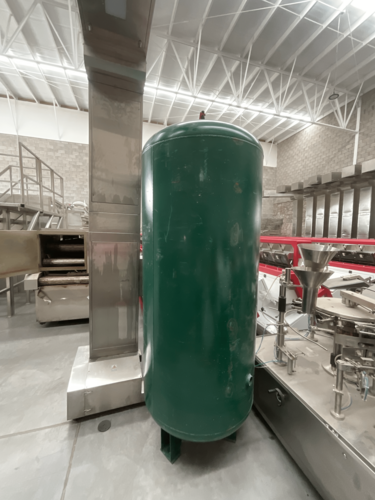
\includegraphics[width=  .5\linewidth]{images/foto/1.png}

% )))

\section{Secador de aire caliente.} % (((
% \includegraphics[width=  \linewidth]{images/decript/2.png}
% \includegraphics[width=  .5\linewidth]{images/foto/2.png}

% )))

\section{Polipasto eléctrico.} % (((


\includegraphics[width=  \linewidth]{images/decript/3.png}

\includegraphics[width=  .5\linewidth]{images/foto/3.png}


% )))

\section{Maquina embollsadora.} % (((

% \includegraphics[width=  \linewidth]{images/decript/4.png}
% \includegraphics[width=  .5\linewidth]{images/foto/4.png}


% )))

\section{Maquina seleccionadora de granos.} % (((
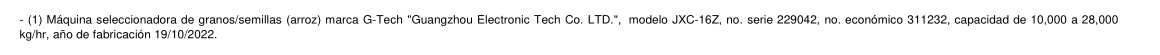
\includegraphics[width=  \linewidth]{images/decript/5.png}
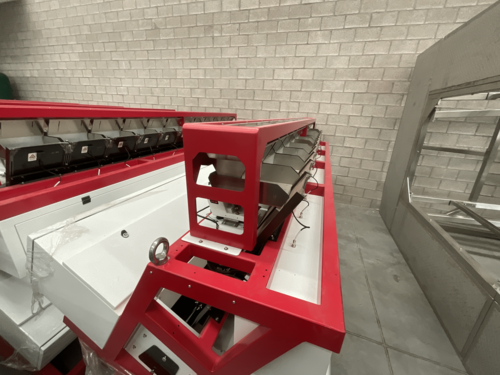
\includegraphics[width=  .5\linewidth]{images/foto/5.png}

% )))

\section{Maquina seleccionadora de granos con plataforma.} % (((

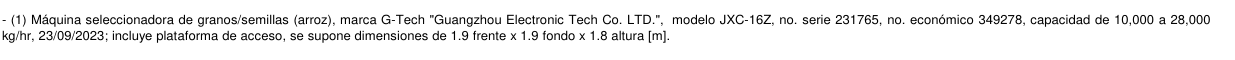
\includegraphics[width=  \linewidth]{images/decript/6.png}
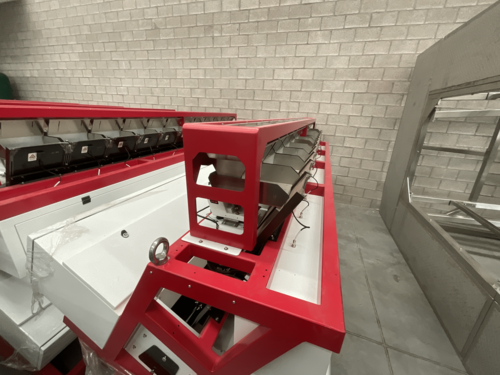
\includegraphics[width=  .5\linewidth]{images/foto/6.png}


% )))

\section{Bombo batidor.} % (((

\includegraphics[width=  \linewidth]{images/decript/7.png}
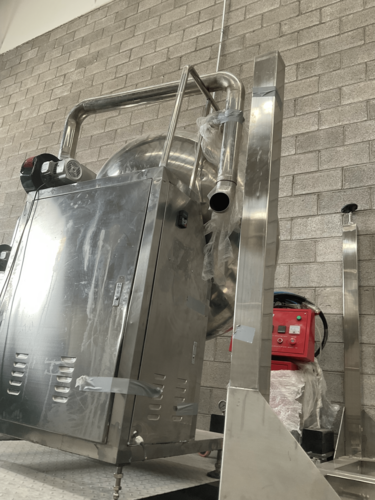
\includegraphics[width=  .5\linewidth]{images/foto/7.png}


% )))

\section{Compresor de aire oil-free.} % (((
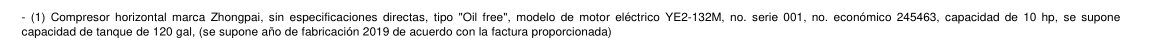
\includegraphics[width=  \linewidth]{images/decript/8.png}
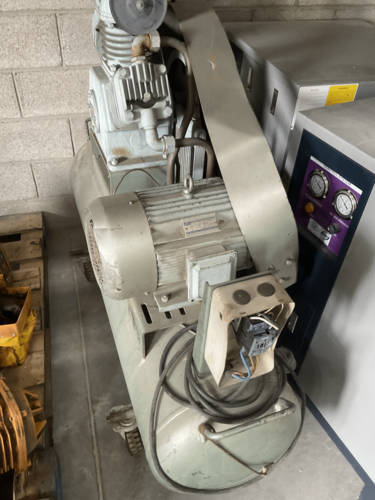
\includegraphics[width=  .5\linewidth]{images/foto/8.png}


% )))

\section{Maquina de aspersión de poliuretano.} % (((

\includegraphics[width=  \linewidth]{images/decript/9.png}
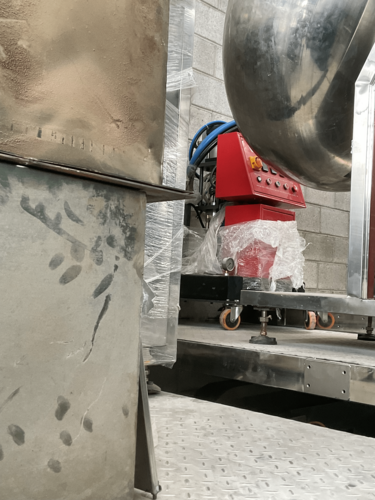
\includegraphics[width=  .5\linewidth]{images/foto/9.png}


% )))

\section{Secador de aire refrigerado.} % (((
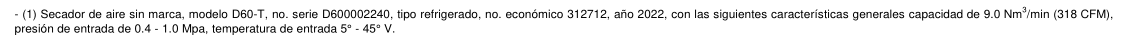
\includegraphics[width=  \linewidth]{images/decript/10.png}
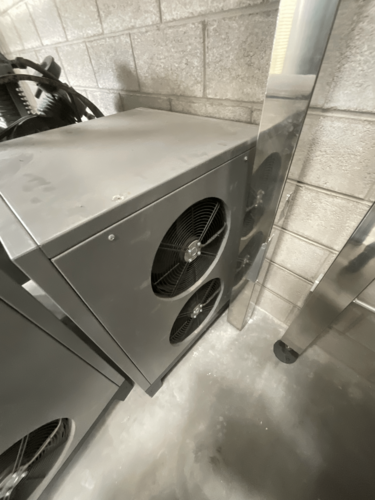
\includegraphics[width=  .5\linewidth]{images/foto/10.png}


% )))

\section{Compresor tipo tornillo.} % (((
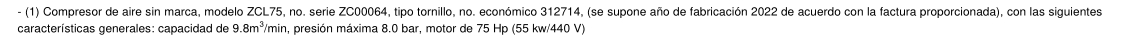
\includegraphics[width=  \linewidth]{images/decript/11.png}
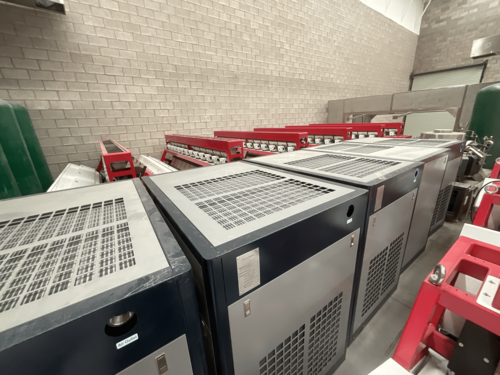
\includegraphics[width=  .5\linewidth]{images/foto/11.png}


% )))

\section{Línea embasadora, con 24 cabezales.} % (((
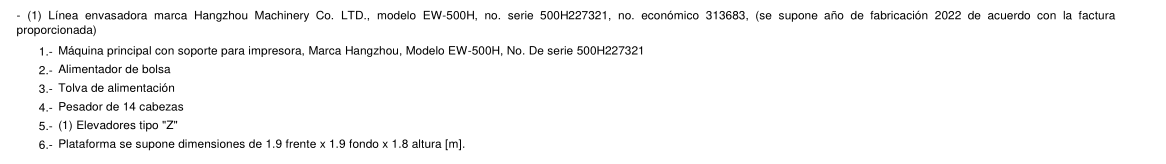
\includegraphics[width=  \linewidth]{images/decript/13.png}
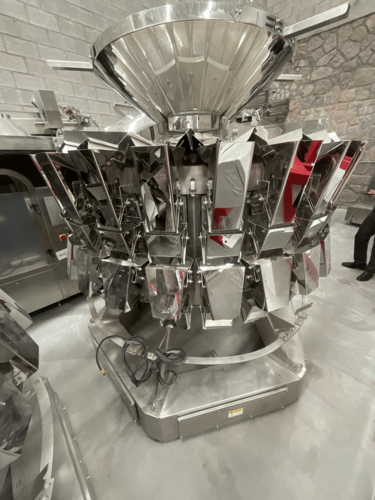
\includegraphics[width=  .5\linewidth]{images/foto/13.png}
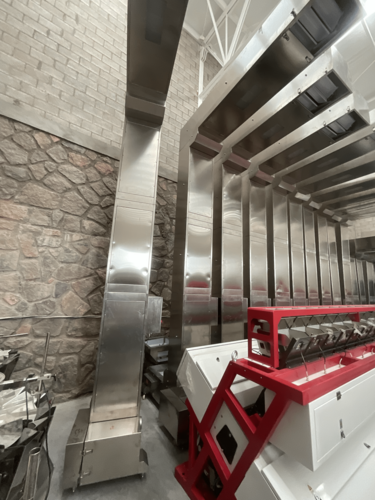
\includegraphics[width=  .5\linewidth]{images/foto/13.1.png}

% )))

\section{Línea embasadora, con 14 cabezales.} % (((
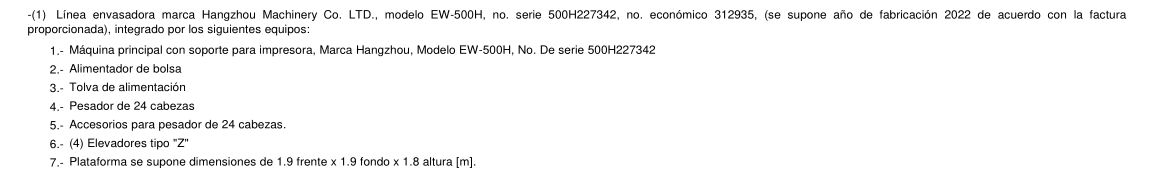
\includegraphics[width=  \linewidth]{images/decript/12.png}
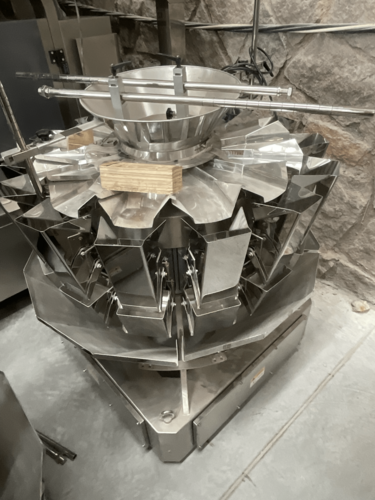
\includegraphics[width=  .5\linewidth]{images/foto/12.png}
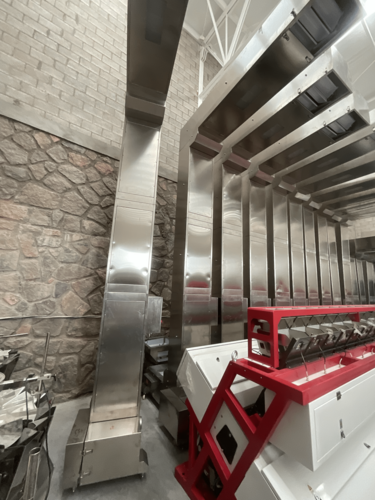
\includegraphics[width=  .5\linewidth]{images/foto/13.1.png}


% )))

\end{document}
